\chapter{\ifproject%
\ifenglish Project Structure and Methodology\else โครงสร้างและขั้นตอนการทำงาน\fi
\else%
\ifenglish Project Structure\else โครงสร้างของโครงงาน\fi
\fi
}

\makeatletter

% \renewcommand\section{\@startsection {section}{1}{\z@}%
%                                    {13.5ex \@plus -1ex \@minus -.2ex}%
%                                    {2.3ex \@plus.2ex}%
%                                    {\normalfont\large\bfseries}}

\makeatother
%\vspace{2ex}
% \titleformat{\section}{\normalfont\bfseries}{\thesection}{1em}{}
% \titlespacing*{\section}{0pt}{10ex}{0pt}

\section{โครงสร้างโดยรวมของโครงงาน (project overview) }
\begin{mypara}
    \indent โครงงานนนี้เป็นระบบสนับสนุนการตัดสินใจสำหรับการวางแผนระบบขนส่งสาธารณะ 
    โดยจะจัดทำเป็นเว็บแอพลิเคชั่นสำหรับการจำลอง และมีการสรุปผลลัพธ์ที่ได้จากการจำลองในรูปแบบทางสถิติ
    ซึ่งในการทำงานของระบบนี้จะมี 4 องค์ประกอบหลักดังนี้  
    
\end{mypara}

% --- Overview figure: placed to appear before the `input` subsection and scaled to fit page ---
\begin{figure}
% width=\textwidth keeps it within the text block; height limits it to most of the page height
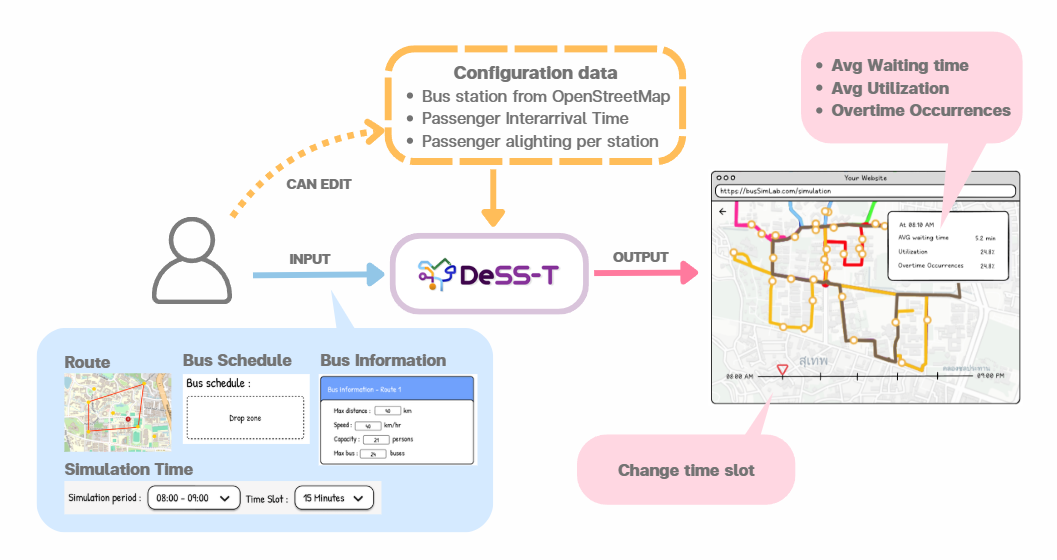
\includegraphics[width=\textwidth,height=0.9\textheight,keepaspectratio]{overview.png}
\caption[Poem]{แผนภาพโดยรวมของโครงงาน}
\label{fig:overview}
\end{figure}

\subsection{input}
  \indent จะเป็นส่วนที่รับข้อมูลจากผู้ใช้ที่จะมีการเปลี่ยนแปลงอยู่เสมอ ได้แก่ เส้นทางการให้บริการของรถ 
  ตารางการเดินรถ และช่วงเวลาที่ต้องการนำมาจำลอง ข้อมูลของรถ

\subsection{configuration data}
  \indent จะเป็นส่วนของข้อมูลที่ใช้เป็นพื้นฐานในการจำลองซึ่งจะไม่ค่อยมีการเปลี่ยนแปลงบ่อย 
  ได้แก่ ข้อมูลการมาถึงสถานีของผู้โดยสาร ข้อมูลการลงรถของผู้โดยสาร ตำแหน่งของสถานี ข้อมูลระยะทางระหว่างสถานี
  
\subsection{simulation engine}
  \indent จะเป็นส่วนที่ทำหน้าที่ในการจำลองระบบขนส่งสาธารณะโดยรถบัสตามข้อมูลที่ได้รับจากส่วน input 
  และ configuration data ซึ่งจะใช้เทคนิคการจำลองแบบเหตุการณ์ไม่ต่อเนื่อง (discrete-event simulation) 
  ในการจำลองระบบขนส่งสาธารณะโดยรถบัส

\subsection{output}
  \indent จะเป็นส่วนที่แสดงผลลัพธ์ที่ได้จากการจำลอง

\section{ ขั้นตอนการทำงาน (Process Overview)}
\begin{mypara}
    \indent โครงงานนี้ทำงานโดยการนำข้อมูลจากผู้ใช้ (input) มาจำลองระบบขนส่งสาธารณะ 
    โดยอ้างอิงข้อมูลพื้นฐานจาก configuration data ซึ่งประกอบด้วยข้อมูลสถานี ข้อมูลระยะทางระหว่างสถานี 
    และข้อมูลพฤติกรรมของผู้โดยสาร หลังจากนั้นระบบจำลอง (simulation engine) จะประมวลผล 
    โดยใช้เทคนิคการจำลองแบบเหตุการณ์ไม่ต่อเนื่อง (discrete-event simulation) 
    เพื่อสร้างผลลัพธ์เชิงสถิติที่แสดงถึงประสิทธิภาพและความหนาแน่นของระบบขนส่ง 
\end{mypara}

\section{User Interface (UI)}
\begin{mypara}
    \indent โครงงานนี้มีการออกแบบส่วนติดต่อผู้ใช้ (User Interface: UI) 
    เพื่อให้ผู้ใช้สามารถป้อนข้อมูลที่จำเป็นสำหรับการจำลองระบบขนส่งสาธารณะได้อย่างง่ายดาย 
    โดย UI จะประกอบด้วยฟอร์มสำหรับกรอกข้อมูลเส้นทางการให้บริการของรถ ตารางการเดินรถ 
    และช่วงเวลาที่ต้องการนำมาจำลอง นอกจากนี้ยังมีการแสดงผลลัพธ์ที่ได้จากการจำลองในรูปแบบกราฟและตารางสถิติ 
    เพื่อช่วยให้ผู้ใช้สามารถวิเคราะห์และตัดสินใจเกี่ยวกับการวางแผนระบบขนส่งได้อย่างมีประสิทธิภาพ
\end{mypara}

\subsection{การจัดกลุ่มผู้ใช้ (User Grouping)}
\indent โครงงานนี้มีการจัดกลุ่มผู้ใช้เป็น 2 กลุ่มหลัก ได้แก่
\begin{itemize}
    \item ผู้ใช้ที่ลงทะเบียน (Registered Users): กลุ่มนี้เป็นผู้ใช้ที่สร้างบัญชีและเข้าสู่ระบบเรียบร้อยแล้ว 
    สามารถเข้าถึงฟังก์ชันทั้งหมดของระบบ รวมถึงบันทึกการจำลอง การตั้งค่าโปรไฟล์ และการเข้าถึงข้อมูลส่วนตัว
    \item ผู้ใช้ที่ไม่ได้ลงทะเบียน (Guest Users / Unregistered Users): กลุ่มนี้เป็นผู้ใช้ทั่วไปที่ไม่ได้สร้างบัญชี 
    สามารถใช้ระบบจำลองได้แบบจำกัดฟังก์ชัน เช่น ทำการจำลองและดูผลลัพธ์ได้ชั่วคราว 
    แต่ไม่สามารถบันทึกหรือเข้าถึงข้อมูลส่วนตัวได้
\end{itemize}

\section{user flow}

